\section{Image Recognition}

\subsection{Bag of Words Framework}
\begin{frame}{Bag of Words in Text Processing}
	\begin{itemize}
		\item A text is represented as an unordered collection of words

		\begin{columns}
			\column{0.35\textwidth}

				\begin{block}{Dictionary}

					\begin{enumerate}
					  \item  \footnotesize{"John"}
					  \item  \footnotesize{"likes"}
					  \item  \footnotesize{"to"}
					  \item  \footnotesize{"watch"}
					  \item  \footnotesize{"movies"}
					  \item  \footnotesize{"also"}
					  \item  \footnotesize{"football"}
					  \item  \footnotesize{"games"}
					  \item  \footnotesize{"Mary"}
					  \item  \footnotesize{"too"}
					 \end{enumerate}
					
				\end{block}

			\column{0.6\textwidth}

				\begin{block}{Two Sentences}
					\begin{enumerate}
						\item \texttt{John likes to watch movies. Mary likes too.}
						\item \texttt{John also likes to watch football games.}
					\end{enumerate}
				\end{block}

				\begin{block}{Histogram Representations}
					\begin{enumerate}
						\item $[1, 2, 1, 1, 1, 0, 0, 0, 1, 1]$
						\item $[1, 1, 1, 1, 0, 1, 1, 1, 0, 0]$
					\end{enumerate}
				\end{block}
		\end{columns}
	\end{itemize}

\end{frame}

\begin{frame}{Bag of Words in Image Recognition}
	\begin{enumerate}
		\item Extract \alert{SIFT} features from each image
		\item Build up \alert{visual vocabulary} from SIFT features of images
		\item Construct a \alert{pyramid} of three levels for each image
		\item \alert{Classify} based on pyramid representations of images
	\end{enumerate}
\end{frame}

\begin{frame}{1. Extract SIFT features from each image}
\begin{itemize}
	\item Various features of images - global and local
	\item Scale Invariant Feature Transform (SIFT)
		\begin{enumerate}
			\item Locate interest points
				\begin{columns}
					\column{0.65\textwidth}
						\begin{equation}
						D(x, y, \sigma) = (G(x, y, k\sigma) - G(x, y, \sigma)) * I(x, y)
						\end{equation}
					\column{0.5\textwidth}
						\begin{figure}[!ht]
							\centering
							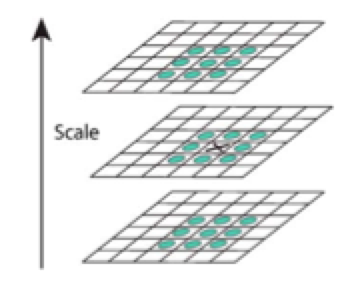
\includegraphics[scale=0.5]{./sift1.png}
						\end{figure}

				\end{columns}
			\item Describe located interest points
				\begin{figure}[!ht]
					\centering
					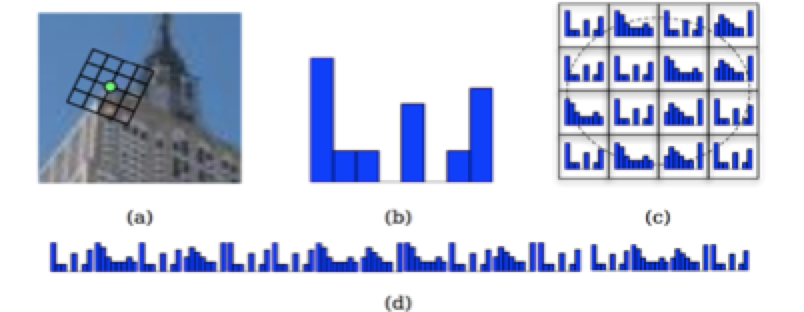
\includegraphics[scale=0.5]{./sift2.png}
				\end{figure}
		\end{enumerate}
\end{itemize}
\end{frame}

\begin{frame}{2. Build up visual vocabulary}

	\begin{algorithm}[H]
	  \caption{Basic K-means Algorithm}
	  \begin {algorithmic}[1]
	  \State Randomly select K points as the initial centroids
	  \Do 
	    \State Form K clusters by assigning all points to their closest centroids.
	    \State Recompute the centroid of each cluster
	  \doWhile Centroids are changed
	  \end{algorithmic}
	\end{algorithm}


	\begin{figure}[!ht]
		\centering
		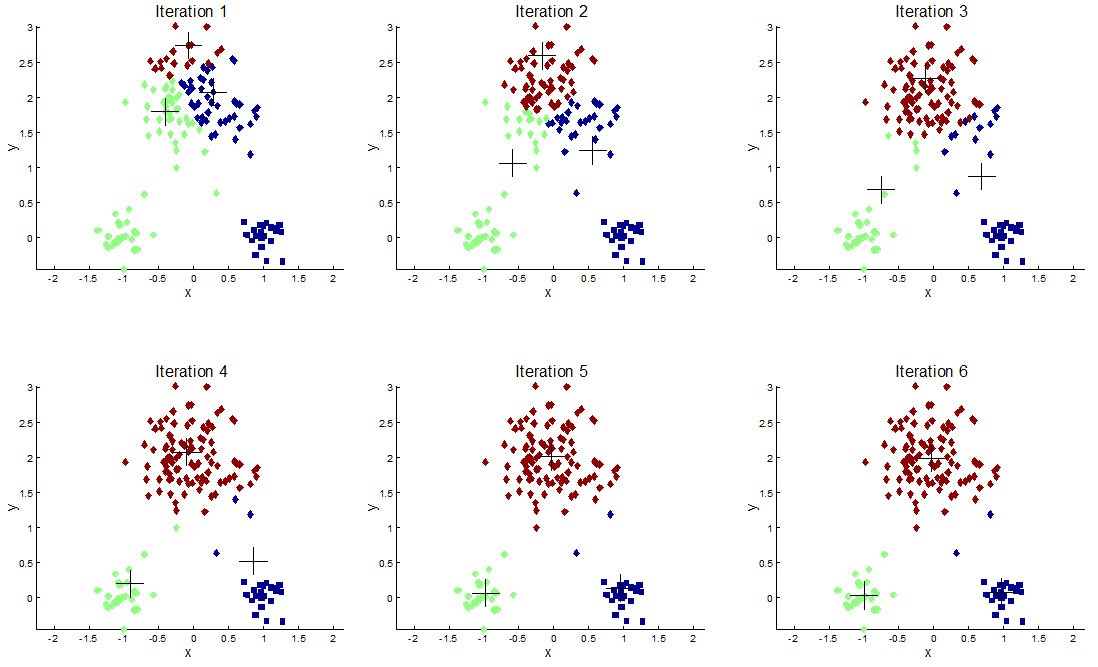
\includegraphics[scale=0.5]{./cluster.jpg}
	\end{figure}

\end{frame}

\begin{frame}{2. Build up visual vocabulary}

	\begin{columns}
		\column{0.5\textwidth}{Build vocabulary through clustering}
			\begin{figure}[!ht]
				\centering
				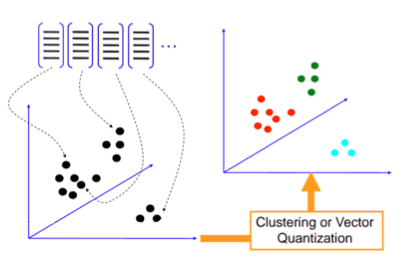
\includegraphics[scale=0.4]{./visualVoc.png}
			\end{figure}

			
			\begin{block}{Vocabulary}
			\centering
					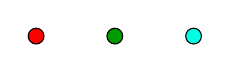
\begin{tikzpicture}
						\draw[fill = red] (0,0) circle (0.1);
						\draw[fill = black!40!green] (1,0) circle (0.1);
						\draw[fill = green!10!cyan] (2,0) circle (0.1);
					\end{tikzpicture}
			\end{block}

		\column{0.5\textwidth}{Project an image into a histogram}
			\begin{figure}[!ht]
				\centering
				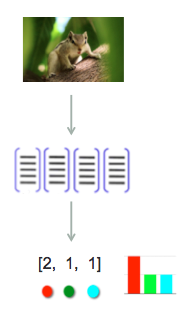
\includegraphics[scale=0.5]{./histogram.png}
			\end{figure}

	\end{columns}

\end{frame}


\begin{frame}{3. Construct a pyramid of three levels}
			
			\begin{figure}[!ht]
				\centering
				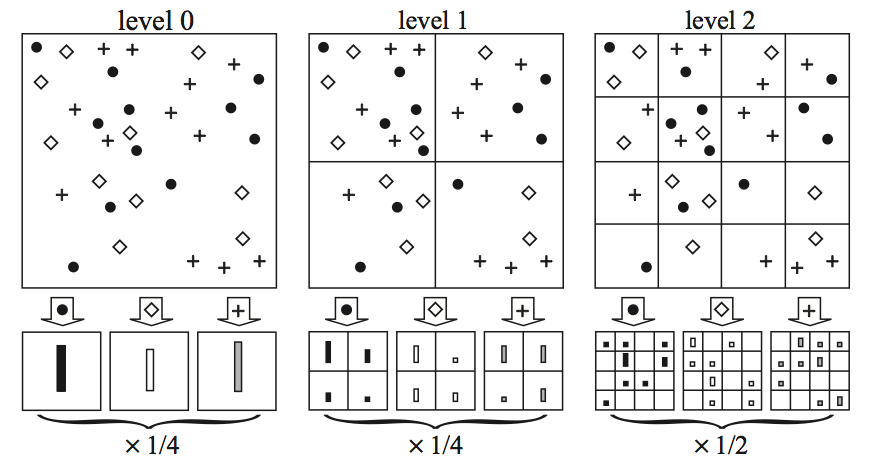
\includegraphics[scale=0.5]{./SpatialPyramidMatch.png}
			\end{figure}

			\begin{equation}
			 weight(l) = \left\{ 
			\begin{array}{l l}
			  \frac{1}{2^L} & \quad \text{$if \ l = 0$ }\\
			  \frac{1}{2^{L-l+1}} & \quad \text{$Otherwise$}
			\end{array} \right.
			\end{equation}

\end{frame}

\subsection{Classification}
\begin{frame}{4. Classify}

	\begin{columns}
		\column{0.5\textwidth}{K Nearest Neighbour (KNN)}



		\column{0.5\textwidth} {Support Vector Machine (SVM)}

	\end{columns}

	
	\begin{columns}
		\column{0.5\textwidth}
			\begin{figure}[!ht]
				\centering
				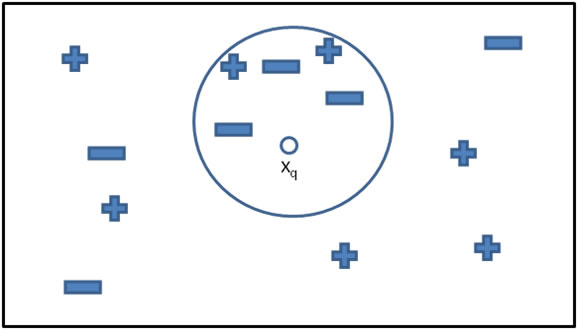
\includegraphics[scale=0.25]{./knn.jpg}
			\end{figure}


		\column{0.5\textwidth} 
			\begin{figure}[!ht]
				\centering
				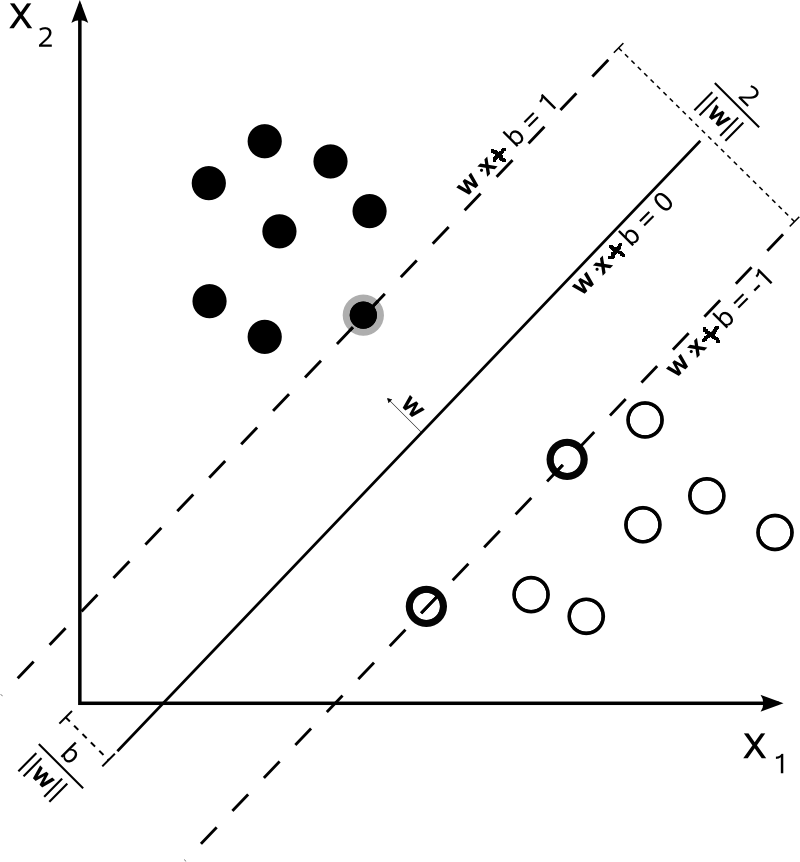
\includegraphics[scale=0.15]{./svm.png}
			\end{figure}
	\end{columns}

\end{frame}

\begin{frame}{Support Vector Machine: Linear Classification}
	\begin{itemize}
		\item Find an optimal hyperplane $y = \mathbf{w} \mathbf{x} + b$  which separates a linearly separable dataset: ${(x_{1}, y_{1}), (x_{2}, y_{2}), ..., (x_{n}, y_{n})}$ where $x \in R^{D}$ and $y \in  \{ -1, +1 \}$

		\item Maximize the distance from support vectors to the hyperplane $\frac{2}{\norm{\mathbf{w}}}$
		  \begin{eqnarray}
		  & \text{minimize} \quad J(\mathbf{w}) = \frac{1}{2} \norm{\mathbf{w}}^2 \nonumber \\
		  & \text{subject to} \quad y_i (\mathbf{w}^{T} x_i + b) \ge 1 \quad \forall i
		  \end{eqnarray}

		\item After introducing Lagrangian, the optimization becomes
		  \begin{eqnarray}
		  & \hat{\boldsymbol{\alpha}} = \argmax{\boldsymbol{\alpha}} \sum_i \alpha_i - \frac{1}{2} \sum_{i,j} y_i y_j \alpha_i \alpha_j x_i^{T} x_j \nonumber\\
		  & \text{subject to} \quad \alpha_i \ge 0  \quad \text{and} \quad \sum_{i=1}^{N} \alpha_i y_i = 0
		  \end{eqnarray}

		\item Final decision function
		  \begin{equation}
		  f(x) = \text{sign}\bigg(\sum_i y_i \alpha_i x_i^T x + b\bigg)
		  \end{equation}
	\end{itemize}
\end{frame}

\begin{frame}{Support Vector Machine: Non-linear Classification}

	\begin{itemize}
	\item Training data appears as dot products $x_i^T x_j$ in equation (4)
	\item Change $x_i^T x_j$ into other forms of kernel function
		\begin{enumerate}
			\item Project training data into higher dimensional space
			\item Perform classification in higher dimensional space
		\end{enumerate}
	\item Decision function is modified to be 
		  \begin{equation}
		  f(x) = \text{sign}\bigg(\sum_i y_i \alpha_i K(x_i,x) + b\bigg)
		  \end{equation}
	\item Some popular kernel functions \begin{columns}
		\column{0.5\textwidth}
			    \begin{table}[!ht]
			        \begin{center}
			        \scalebox{0.75}{
			          \begin{tabular}{cc}
			          \hline
			          \head{Kernel type} & \head{Kernel function}\\
			          \hline
			          Linear & $x_i^T x_j$ \\
			          Polynomial & $(\gamma x_i^T x_j + r)^d$ \\ 
			          RBF (Gaussian) & $\exp(-\gamma \norm{x_i - x_j}^2)$ \\ 
			          Sigmoid & $\tanh(\gamma x_i^T x_j + r)$ \\ 
			          Histogram intersection \cite{barla2003histogram} &  $\sum_{p = 1}^{D} min(x_i^p, x_j^p)$ \\
			          \hline
			          \end{tabular}
			        }
			        \end{center}
			        \caption{Kernel functions}
			    \end{table}

		\column{0.6\textwidth}
			\begin{figure}[!ht]
				\centering
				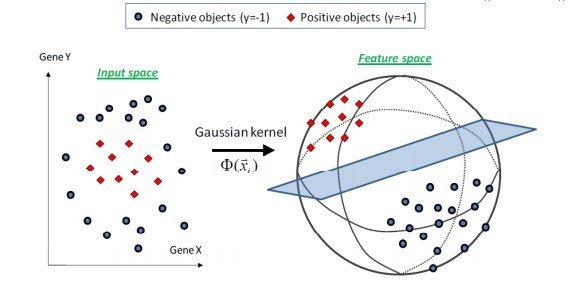
\includegraphics[scale=0.4]{./rbf.jpg}
			\end{figure}
	\end{columns}
	\end{itemize}
\end{frame}

\subsection{Experiments}
\begin{frame}{Experiments of Image Recognition}
\begin{itemize}
	\item Data set: 60 images from 6 classes
			\begin{figure}[!ht]
				\centering
				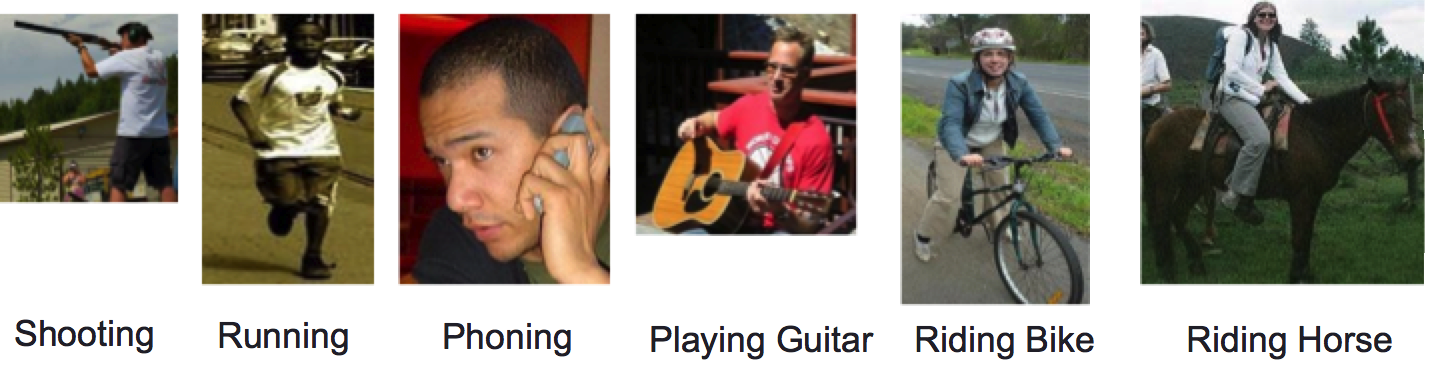
\includegraphics[scale=0.14]{./imageSet.png}
			\end{figure}
	\item Evaluation metric: recognition accuracy $ = \frac{\text{correct predictions}}{\text{number of testing samples}}$
	
	\begin{table}[!ht]
    \begin{center}
    	\scalebox{0.6}{
      \begin{tabular} {cccc}
      \hline
    	\head{SVM} & \head{One-level} & \head{Two-level} & \head{Three-level}\\
      \hline
      Linear & 74.17 & 80 & {\bf 87.5} \\
      Poly & 70 & 62.5 & 31.67 \\
      RBF & 37.5 & 83.33 & 74.17 \\
      Sigmoid & 16.67 & 16.67 & 16.67 \\
      Histogram Intersection & 79.17 & 82.5 & {\bf 85} \\
      \hline
      \end{tabular}
    }
    \end{center}
    \caption{Recognition accuracies (percent) using SVM}
	\end{table}

	\begin{table}[!ht]
	\begin{center}
    	\scalebox{0.6}{
	  \begin{tabular} {cccc}
	  \hline
		\head{} & \head{One-level} & \head{Two-level} & \head{Three-level}\\
	  \hline
      KNN & 50.83 & 45 & 48.33 \\
      \hline
      \end{tabular}
    }
    \end{center}
    \caption{Recognition accuracies (percent) using KNN}
\end{table}

\end{itemize}
\end{frame}

